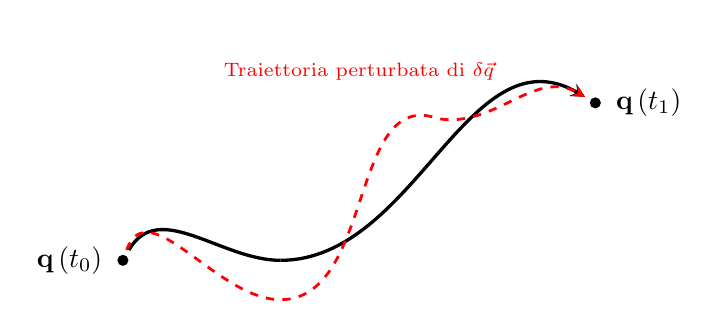
\begin{tikzpicture}[>=stealth, thick, scale=1.0]

% Punti A e B
\node[label=left:{$\mathbf{q}\left(t_0\right)$}] (A) at (0,0) {};
\node[label=right:{$\mathbf{q}\left(t_1\right)$}] (B) at (6,2) {};

% Traiettoria principale (nera)
\draw[line width=1.2pt] (A) to[out=60, in=180] (2,0);
\draw[->, line width=1.2pt] (2,0) to[out=0, in=150] (B);

% Curva perturbata (rossa, composta da 3 tratti curvi)
\draw[->, red, dashed, line width=1pt]
  (A)
    to[out=70, in=180] (2,-0.5)
    to[out=0, in=160] (4,1.8)
    to[out=-10, in=150] (B);

% Punti visibili
\fill (A) circle (2pt);
\fill (B) circle (2pt);

% Etichetta facoltativa
\node[red] at (3,2.4) {\scriptsize Traiettoria perturbata di $\delta\vec{q}$ };

\end{tikzpicture}